% This is part of Un soupçon de mathématique sans être agressif pour autant
% Copyright (c) 2012-2013
%   Laurent Claessens
% See the file fdl-1.3.txt for copying conditions.

% Ce fichier est celui pour les premières STMG.

\begin{center}

           \ifpdf
            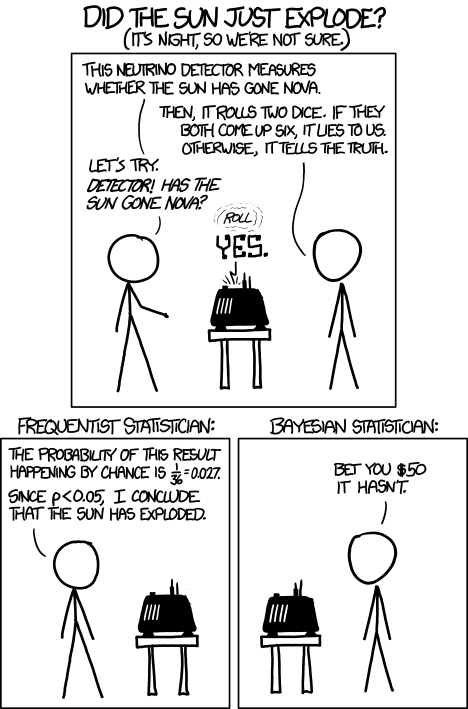
\includegraphics[width=8cm]{frequentists_vs_bayesians.png}
        \else
            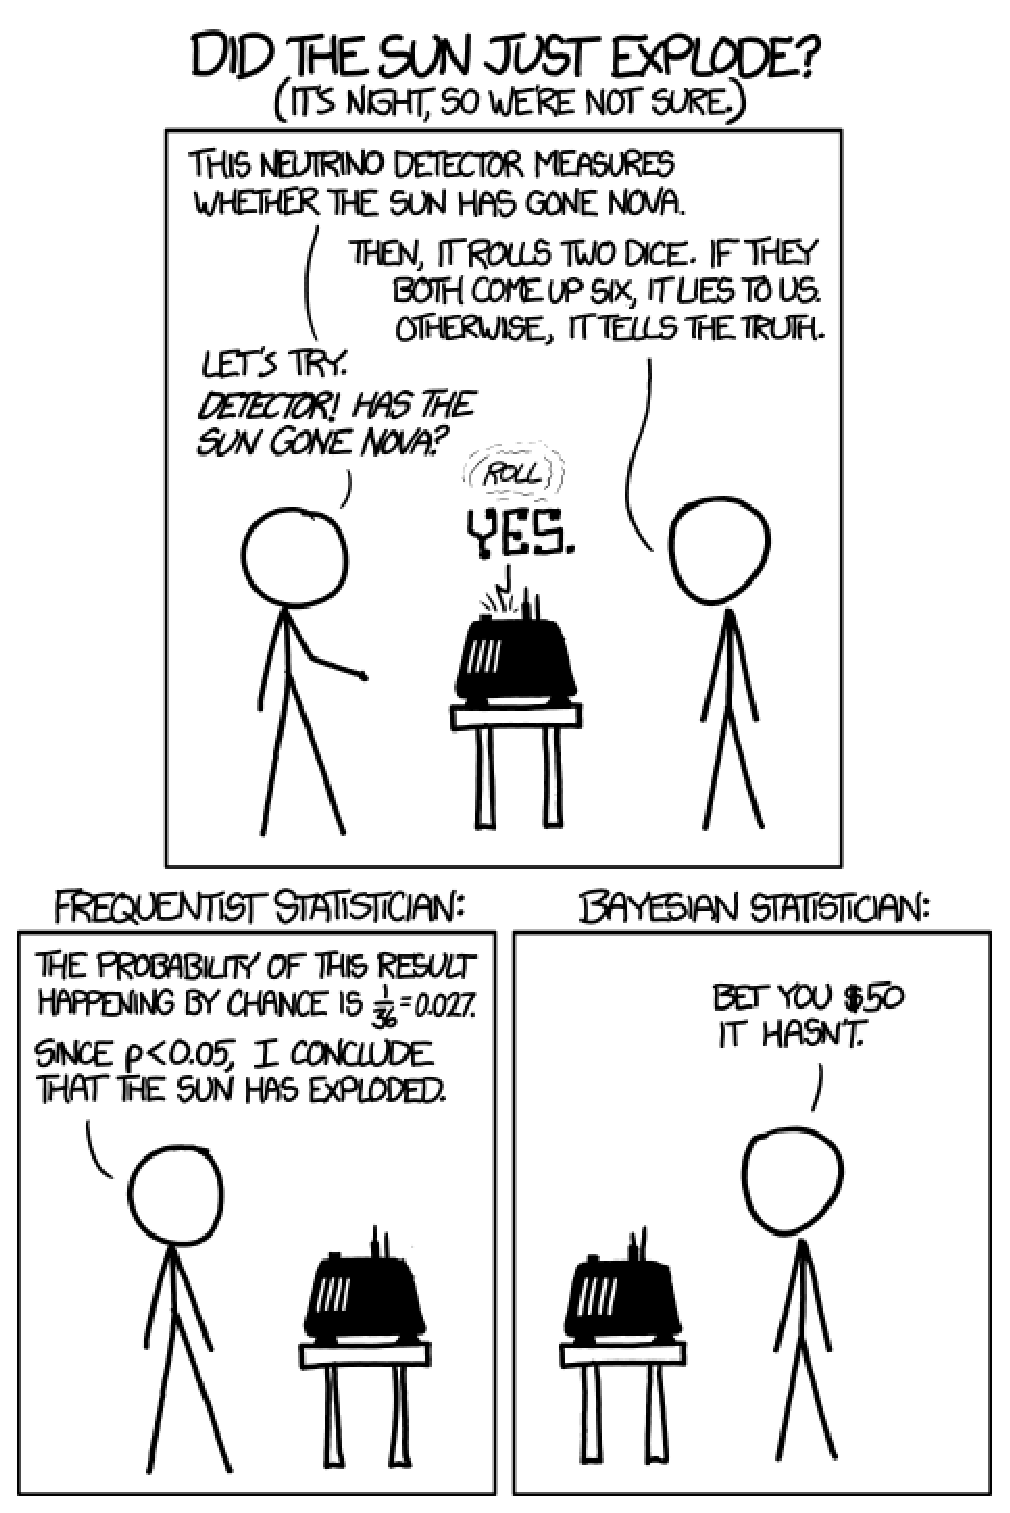
\includegraphics[width=8cm]{frequentists_vs_bayesians.eps}

            \fi

            \url{http://xkcd.com/1132/}, image publiée sous licence \href{http://xkcd.com/license.html}{CreativeCommons}.

\end{center}

Une chouette page concernant les intervalles de confiance à propos de l'élection à l'UMP est celle-ci :\\
\url{http://david.monniaux.free.fr/dotclear/index.php/post/2012/11/23/Le-sens-statistique-de-l-élection-à-l-UMP}

%+++++++++++++++++++++++++++++++++++++++++++++++++++++++++++++++++++++++++++++++++++++++++++++++++++++++++++++++++++++++++++ 
\section{Intervalle de fluctuation}
%+++++++++++++++++++++++++++++++++++++++++++++++++++++++++++++++++++++++++++++++++++++++++++++++++++++++++++++++++++++++++++

Cette section provient de \cite{JqcbOc}.

Un médecin voudrait savoir si le pourcentage d'habitants atteints d'hypertension artériel dans sa région est normal, sachant qu'une étude récemment publiée donne un pourcentage de \( 16\%\) pour d'autres régions comparables. Nous notons \( p\) la proportion (inconnue) d'hypertendus dans la région et nous constituons un échantillon de \( n=100\) habitants de la région. Nous notons \( f\) la fréquence des hypertendus dans l'échantillon.

Bien entendu, si la population est normale, le nombre \( f\) ne devrait pas être trop loin de \( 0.16\) -- à moins d'un coup de malchance dans la sélection de l'échantillon. Voyons cela de plus près.

Nous formulons l'hypothèse que la proportion des hypertendus est bien \( p=0.16\). Dans ce cas si nous désignons par \( X\) le nombre d'hypertendus dans l'échantillon, c'est une variable aléatoire binomiale de paramètres \( n=100\) et \( p=0.16\).

Toute la difficulté est évidemment maintenant de définir ce que nous appelons «normal». Pour donner une idée, voici les probabilités de la binomiale de paramètres \( n=100\), \( p=0.16\).

%The result is on figure \ref{LabelFigJRVlexw}. % From file JRVlexw
%\newcommand{\CaptionFigJRVlexw}{<+Type your caption here+>}
\begin{center}
\input{Fig_JRVlexw.pstricks}
\end{center}

La règle que nous allons retenir pour dire si une situation est «normale» est la suivante :
\begin{Aretenir}
    Une situation est «anormale» si elle a mois de \( 5\%\) de chance de s'expliquer par un coup de chance (ou de malchance, suivant le point de vue). Nous allons donc déclarer que les \( 2.5\%\) les plus à gauche et les \( 2.5\%\) les plus à droite sont anormaux.
\end{Aretenir}
Bien entendu dans le cas de notre médecin, avoir un nombre anormalement élevé de personnes en bonne santé n'est pas une \emph{mauvaise} nouvelle. 

Nous allons chercher des bornes \( a\) et \( b\) telles que \emph{au moins} \( 95\%\) des probabilités soient entre \( a\) et \( b\). Au niveau du dessin, ça donne ceci :


%The result is on figure \ref{LabelFigYVZAXhU}. % From file YVZAXhU
%\newcommand{\CaptionFigYVZAXhU}{<+Type your caption here+>}
\begin{center}
\input{Fig_YVZAXhU.pstricks}
\end{center}
Les zones rouges sont considérées comme anormales. En d'autres termes :
\begin{enumerate}
    \item
        Si sur l'échantillon de \( 100\) personnes prises dans la population le médecin observe \( 8\) ou moins sont atteintes d'hypertension, alors le médecin dira que sa région est en anormalement bonne santé. Il ne s'inquiétera pas, et ça fera un très bon thème de campagne de publicité pour les producteurs du fromage local.
    \item
        Si le nombre d'hypertendu est entre \( 9\) et \( 23\), le médecin dira qu'il n'y a rien de particulier à signaler.
    \item
        Si le nombre d'hypertendu est égal ou supérieur à \( 24\), alors la marque locale de fromage ne s'en vantera pas trop et le médecin essayera de comprendre ce qui ne fonctionne pas.
\end{enumerate}
L'intervalle entre \( 9\) et \( 23\) est nommé l'\defe{intervalle de fluctuation}{intervalle!fluctuation!de première}.

%+++++++++++++++++++++++++++++++++++++++++++++++++++++++++++++++++++++++++++++++++++++++++++++++++++++++++++++++++++++++++++ 
\section{Exercices}
%+++++++++++++++++++++++++++++++++++++++++++++++++++++++++++++++++++++++++++++++++++++++++++++++++++++++++++++++++++++++++++

\Exo{smath-0380}
\Exo{smath-0383}
\Exo{smath-0384}

%+++++++++++++++++++++++++++++++++++++++++++++++++++++++++++++++++++++++++++++++++++++++++++++++++++++++++++++++++++++++++++ 
\section{À l'ordinateur}
%+++++++++++++++++++++++++++++++++++++++++++++++++++++++++++++++++++++++++++++++++++++++++++++++++++++++++++++++++++++++++++

\Exo{smath-0385}
